\documentclass[uplatex,dvipdfmx,a4paper,10pt,twoside,openany,onecolumn]{jsbook}
\usepackage{graphicx}
\usepackage{listings}
\usepackage{datetime}

%% Font Config
\usepackage[deluxe]{otf}
\usepackage[noalphabet,ipaex]{pxchfon}
\usepackage[prefernoncjk]{pxcjkcat}
\usepackage[utf8]{inputenc}
\usepackage[T1]{fontenc}
\usepackage{textcomp}
\usepackage{lmodern}
\usepackage{fix-cm}
\cjkcategory{sym18}{cjk}
\cjkcategory{sym19}{cjk}

%% Cites
\usepackage{cite}
\makeatletter
\def\NAT@parse{\typeout{}}
\makeatother

%% Margin Config
\usepackage[dvipdfm,top=10zw,bottom=12zw,left=10zw,right=10zw]{geometry}

\newcommand{\parasep}{\vspace*{3zh}}
\setlength{\footskip}{30pt}
\renewcommand{\baselinestretch}{1.25}
\sloppy

%% Link Config
\PassOptionsToPackage{hyphens}{url}
\usepackage[bookmarks=true,bookmarksnumbered=true,colorlinks=true,pdfusetitle=true]{hyperref}
\usepackage{pxjahyper}
\hypersetup{
  linkcolor=black,
  citecolor=black,
  filecolor=black,
  urlcolor=black,
  anchorcolor=black
}

%% Header Config
\usepackage{fancyhdr}
\pagestyle{fancy}
\lhead{\gtfamily\sffamily\bfseries\upshape \leftmark}
\chead{}
\rhead{\gtfamily\sffamily\bfseries\upshape \rightmark}
\fancyfoot[CE,CO]{\thepage}
\fancypagestyle{plainhead}{%
\fancyhead{}
\renewcommand{\headrulewidth}{0pt}
\renewcommand{\footrulewidth}{0pt}}
\renewcommand{\sfdefault}{phv}

\renewcommand{\sectionmark}[1]{\markright{\thesection~#1}{}}
\renewcommand{\chaptermark}[1]{\markboth{\prechaptername\ \thechapter\ \postchaptername~#1}{}}
\renewcommand{\headfont}{\gtfamily\sffamily\bfseries}

\makeatletter
%% MakeTile Config
\def\thesis#1{\gdef\@thesis{#1}}
\def\affiliation#1{\gdef\@affiliation{#1}}
\def\studentid#1{\gdef\@studentid{#1}}
\def\supervisor#1{\gdef\@supervisor{#1}}

\def\enTitle#1{\gdef\@enTitle{#1}}
\def\enAuthor#1{\gdef\@enAuthor{#1}}
\def\enDate#1{\gdef\@enDate{#1}}
\def\enThesis#1{\gdef\@enThesis{#1}}
\def\enAffiliation#1{\gdef\@enAffiliation{#1}}
\def\enStudentid#1{\gdef\@enStudentid{#1}}
\def\enSupervisor#1{\gdef\@enSupervisor{#1}}

\renewcommand{\maketitle}{%
\begin{titlepage}
\begin{center}
\vspace*{120truept}
{\Large \@thesis}\\

\vspace*{30truept}
{\huge \@title}\\ % タイトル
\vspace*{10truept}
{\Large \@enTitle}\\ % タイトル

\vspace*{20truept}
{\Large 指導教官\hspace*{20truept}\@supervisor}\\

\vspace{20truept}
{\Large \@date}\\

\vspace{100truept}
{\Large \@affiliation}\\

\vspace{50truept}
{\Large 学籍番号: \@studentid}\\ % 学籍番号

\vspace{10truept}
{\huge \@author}\\ % 著者

\end{center}
\end{titlepage}
}
\makeatother

%% Document Config
\studentid{9092153232}

\title{飛行機における入力値抽出手法の提案}
\author{山田 太郎}
\affiliation{例示大学 数理科学部\\
ポストインターネット学科}
\date{2099年 3月}
\thesis{2098年度 卒業研究論文}
\supervisor{田中 次郎 教授}

\enTitle{Extracting Input in the Case of Airplanes}
\enAuthor{Taro Yamada}
\enAffiliation{Department of Post-Internet\\
Faculty of Mathematical Sciences\\
at Reiji University}
\enDate{March 2099}
\enThesis{The Graduate Thesis}
\enSupervisor{Prof. Jiro Tanaka}


\begin{document}

\maketitle

\chapter*{概要}
\thispagestyle{empty}
あのイーハトーヴォのすきとおった風,夏でも底に冷たさをもつ青いそら,うつくしい森で飾られたモリーオ市,郊外のぎらぎらひかる草の波.またそのなかでいっしょになったたくさんのひとたち,ファゼーロとロザーロ,羊飼のミーロや,顔の赤いこどもたち,地主のテーモ,山猫博士のボーガント・デストゥパーゴなど,いまこの暗い巨きな石の建物のなかで考えていると,みんなむかし風のなつかしい青い幻燈のように思われます.では,わたくしはいつかの小さなみだしをつけながら,しずかにあの年のイーハトーヴォの五月から十月までを書きつけましょう.

\newpage

\chapter*{Abstract}
\thispagestyle{empty}
Lorem ipsum dolor sit amet, consectetur adipiscing elit, sed do eiusmod tempor incididunt ut labore et dolore magna aliqua. Ut enim ad minim veniam, quis nostrud exercitation ullamco laboris nisi ut aliquip ex ea commodo consequat. Duis aute irure dolor in reprehenderit in voluptate velit esse cillum dolore eu fugiat nulla pariatur. Excepteur sint occaecat cupidatat non proident, sunt in culpa qui officia deserunt mollit anim id est laborum.

\newpage

\frontmatter

\setcounter{tocdepth}{1}
\tableofcontents

\mainmatter

\chapter{テスト文章}\label{sec:first}

Lorem ipsum \cite{LoremipsWikipedia:online} (ロレム・イプサム,略してリプサム lipsum ともいう)とは,出版,ウェブデザイン,グラフィックデザインなどの諸分野において使用されている典型的なダミーテキストである.

\begin{quote}
  Lorem ipsum dolor sit amet, consectetur adipiscing elit, sed do eiusmod tempor incididunt ut labore et dolore magna aliqua. Ut enim ad minim veniam, quis nostrud exercitation ullamco laboris nisi ut aliquip ex ea commodo consequat. Duis aute irure dolor in reprehenderit in voluptate velit esse cillum dolore eu fugiat nulla pariatur.
\end{quote}

デカルト座標で,点 \((a, b)\) を中心とする半径 \(r\) の円は,次式の陰関数で与えられる.

\[
(x - a)^2 + (y - b)^2 = r^2
\label{eq:circle}
\]

図\ref{fig:image} は,Unsplash \footnotemark から引用している.

\footnotetext{\url{https://unsplash.com/}}

\begin{figure}[tb]
\centering
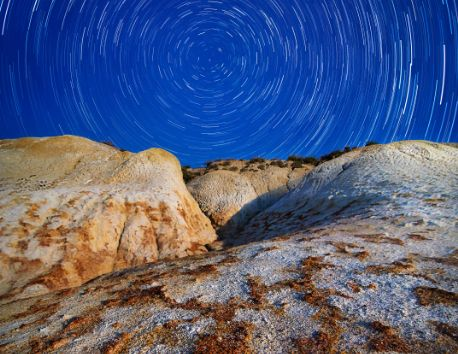
\includegraphics[
  keepaspectratio=true,
  width=0.85\linewidth,
  height=0.15\paperheight
]{../assets/sample.jpg}
\caption{サンプル}
\label{fig:image}
\end{figure}


\backmatter

\chapter*{謝辞}
\markright{謝辞}
\addcontentsline{toc}{chapter}{謝辞}
本研究に手厚いご指導を頂きました田中 次郎教授に深謝いたします.
また,実験では被験者を快く引き受けていただき,
執筆に際しては多くのご指摘をいただきました田中ゼミナールの同期・後輩の皆さまに
心より感謝申し上げます.

\newpage

%% Bibliography
\bibliographystyle{junsrt}
\bibliography{bib/main}

\end{document}
